\paragraph{When has a second line actually opened?}
An outage changes the algebraic map from generator internal voltages
to PMU phasors. PMU-based outage identification already exploits
this dependence on topology \cite{tate2008outage}. Here the issue
is whether a later report represents a new opening, persistence of
an open branch, or its reclosure. The discrete states include the
intact network, 35 non-islanding line outages, and competing fault
and load shunts at the modeled buses. A shunt must compete for the
same observations. If only lines are eligible, a fault can receive
a confident but incorrect line label.
Closing a line restores its branch stamp and leaves the generator
sources continuous. A subsequent opening of the same line is again
an admissible transition.

Let $u$ be the ten complex internal generator phasors divided by
their operating-point values. Let $J$ inject the corresponding
nominal Norton currents, $Y_q$ include generator admittances and
the branch stamps in state $q$, and $C_q$ select eight normalized
voltage phasors and seven normalized, oriented branch-current phasors.
The current row for a measured open branch is zero. Then
\[
 H_q=C_qY_q^{-1}J,\qquad y_k=H_qu_k+\epsilon_k.
\]
We reconstruct current from its bias-corrected magnitude and
relative phase. For the calculation we use proper complex Gaussian
errors with diagonal covariance $R$. Its voltage entries sum the
two quadrature variances. Its current entries combine the fitted
magnitude and angular variances at nominal current. This approximation
discards cross-terminal and temporal correlations in the instrument model.

For each possible transition $q\to r$, condition a local source prior
$u_{k-1}\sim\mathcal{CN}(\mathbf{1},I)$ on the previous PMU report,
then propagate one step with a zero-mean increment of covariance $Q$.
The conditional mean, covariance and next measurement law are
\begin{align*}
 P_q&=(I+H_q^*R^{-1}H_q)^{-1},\\
 m_q&=\mathbf{1}+P_qH_q^*R^{-1}(y_{k-1}-H_q\mathbf{1}),\\
 L_{qr,k}&=\mathcal{CN}\!\left(y_k;H_rm_q,\,
                  R+H_r(P_q+Q)H_r^*\right).
\end{align*}
The working scale $Q=(2\pi\,0.5/30)^2I$ allows source motion
over one reporting interval. Its scale corresponds to a 0.5-Hz
frequency deviation near the operating point. Summing the transition
likelihoods propagates the discrete posterior,
\[
 \pi_k(r)=
 \frac{\sum_q T_{qr}\pi_{k-1}(q)L_{qr,k}}
      {\sum_{q,s}T_{qs}\pi_{k-1}(q)L_{qs,k}} .
\]
This recursion is exact for the stated conditional observation law.
Only the topology probabilities carry the complete PMU history.
The continuous-source calculation restarts from the local prior
for each report pair. The intact state assigns probability $1/720$
per report to a change, shared equally among the line, fault and load
families, then among eligible assets and their strengths. The return
probability per report is $1/40$ for an open line or load change and
$1/12$ for a fault. A torque input can change the internal sources
while leaving the circuit intact.

The four-family monitor supplies the first line declaration.
The topology filter then runs at 30 reports/s. A supported transition
requires posterior probability at least 0.99 and an innovation within
the working complex-Gaussian 0.99999 quantile. A new opening publishes
at the next three-report decision instant if the measurements still
support that line. Persistent openings and reclosures generate no
additional line declaration. A late line proposal whose estimated
onset falls within an already declared opening of that branch is
assigned to the existing episode.
Competing electrical labels with the same estimated onset as an
opening already declared by the filter belong to that transition.

For a proposed fault or load at bus $b$ we also compare continued
switching with an added shunt on the inferred topology. The shunt
changes the observation operator by
\[
 H_{q,b}(d)=H_q-
 \frac{d\,(C_qY_q^{-1}e_b)(e_b^\top Y_q^{-1}J)}
      {1+d\, e_b^\top Y_q^{-1}e_b}.
\]
We average likelihoods over three strengths per load or fault regime,
including weak and nominal fault regimes, on up to three available
reports. A shunt proposal is withheld only when the supported topology
fits and the shunt likelihood ratio is below 0.01 at every available
onset within two reports of the proposed onset. Generator alarms
retain their torque-based decision. This experiment assumes successive
line operations with at most one open line at a time.

Development included 66 additional streams with 150 interventions.
They included repeat openings of the same branch, three successive
openings, faults of two severities, load changes and torque pulses
after a reclosure. The previous and revised estimators made
\SwDevOldJoint{} and \SwDevNewJoint{} exact diagnoses and issued
\SwDevOldExtra{} and \SwDevNewExtra{} unmatched alarms.
In one three-opening sequence the revised estimator located all
three operations and also reported a spurious fault.

\begin{table}[t]\centering\footnotesize
\caption{Paired four-family test of the switch filter. Det.\ counts triggers within 45 reports. Family and exact require a published diagnosis by that deadline. Active counts exact diagnoses before clearance. Extra counts unmatched alarms in all 465 streams. All event counts use 420 as the denominator.}
\label{tab:switch-trial}
\setlength{\tabcolsep}{2.3pt}
\begin{tabular}{lrrrrrr}\toprule
Method & Macro-F1 & Det. & Family & Exact & Active & Extra\\\midrule
Recovery bank & 0.9647 & 402 & 402 & 402 & 384 & 11 \\
Refitted ExtraTrees & 0.6855 & 303 & 253 & 236 & 97 & 1 \\
Current estimator & 0.9737 & 410 & 410 & 410 & 392 & 11 \\
Switch filter & 0.9758 & 410 & 410 & 410 & 392 & 9 \\
\bottomrule\end{tabular}\end{table}

\begin{figure}[t]\centering
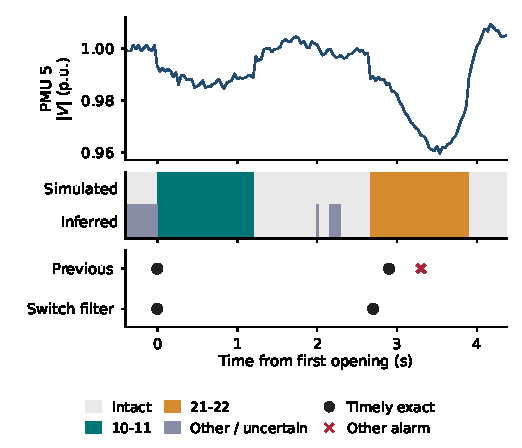
\includegraphics[width=\columnwidth]{figures/generated/line_switch_example.pdf}
\caption{PMU voltage, topology and publication times on a blind
two-opening record. Time zero is the first physical opening.
The middle panel compares the simulated configuration with the
filter's supported mode. Gray-violet includes time before the
first declaration and reports without a supported displayed mode.
The example is the first two-opening record in simulation order on
which the two estimators differ in exact or unmatched counts and the
bank identified the first opening.}
\label{fig:switch-example}
\end{figure}

Table~\ref{tab:switch-trial} gives the independent paired test on
the same reserved asset catalog. The 95\% block-bootstrap interval
for exact event attribution was \SwExactCI{}\%. The interval for the change
in exact diagnoses was $[\SwJointCI]$ percentage points. The interval
for unmatched alarms was $[\SwExtraCI]$ alarms per 15
blocks. Both use 12,000 paired resamples of whole scenario blocks.
As a separate check on reclosure timing, we found the first
supported target line during the second open interval and then
the first supported intact state, allowing early returns to count
as errors. That return fell within three reports of the simulated
reclosure for \SwClosures{} of the 30 second line openings.
Reclosures are internal state changes. The four-family score counts
each line opening as one event.

The six reclosures without a supported opening all involved line
1--39. The full monitor still located the opening through its
existing bank. Across all four families, the two estimators
detected the same \SwNewDetected{} events and gave the correct
family and asset in each. Both missed six generator pulses and
four load changes after a fault. Macro-F1 rose from \SwOldFOne{}
to \SwNewFOne{} because the switch filter issued fewer unmatched
line alarms. Neither estimator emitted an alarm in 165 quiet streams.
